\documentclass{article}
%\documentclass{exam}
\usepackage[italian]{babel}
\usepackage[T1]{fontenc}
\usepackage{graphicx}
\usepackage[utf8x]{inputenc}
\usepackage{amsmath}
\usepackage{amsthm}
\usepackage{hyperref}
\date{Novembre 2015}
\author{Francesco Sacco, Lorenzo Cavuoti}
\title{Usi non lineari dell'OpAmp}

\newcommand{\vz}{V_{sh}(0)}

\begin{document}
	\maketitle		
	\paragraph{1)}
	\subparagraph{a.}
		Abbiamo collegato il circuito e alimentato a $\pm 15V$, i componenti, misurati con il multimetro digitale, risultano:
		\begin{itemize}
			\item $C_T=0.95\pm0.04 nF$
			\item $C_F=1.02\pm0.04 nF$
			\item $R_1=99.7\pm0.8 k\Omega$
			\item $R_2=99.3\pm0.8 \Omega$
			\item $C_1=21.0\pm0.9 nF$
		\end{itemize}
		Il potenziomentro è stato regolato in modo da produrre una tensione $V_P=184.3\pm0.9 mV$ misurata con il multimetro digitale

	\subparagraph{b.}
		Per spiegare il circuito dell'amplificatore di carica è meglio analizzarlo con i suoi due sotto-circuiti separatamente, e poi vedere come si incastrano assieme.\newline

		Il primo sottocircuito è quello che è collegato al voltaggio in ingresso $V_S$, esso si può vedere nella figura \ref{fig:circ1}
		\begin{figure}
			\label{fig:circ1}
			\centering
			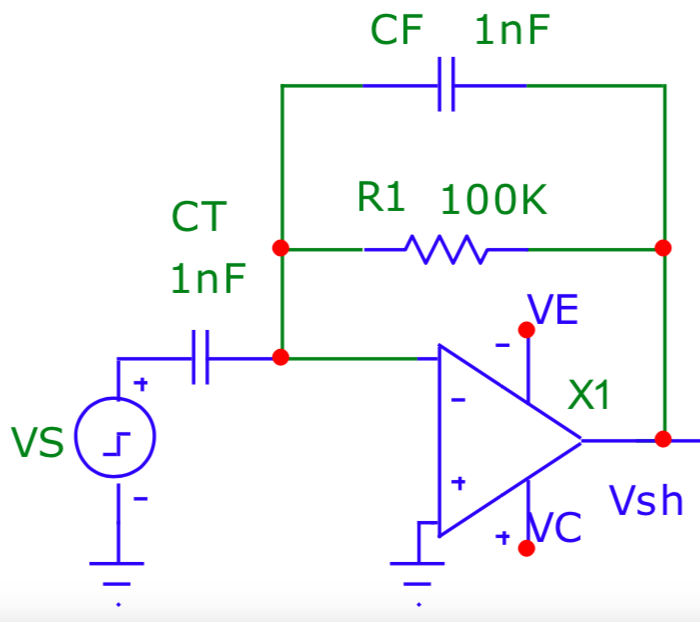
\includegraphics[width=70mm]{immagini/circ1a.png}
			\caption{sotto-circuito 1}
		\end{figure}
		, risolvere il circuito equivale a risolvere questo sistema di 3 equazioni
		\begin{equation}
			\begin{cases}
				V_S-V_-=\frac{Q_T}{C_T}\\
				V_--V_{sh}=I_1R_1\\
				V_--V_{sh}=\frac{Q_F}{C_F}
			\end{cases}
		\end{equation}
		Derivando rispetto al tempo la prima e la terza equazione, supponendo che $\frac{dV_s}{dt}=0$\footnote{visto che è un'onda quadra possiamo supporre di interessarci al circuito nei punti in cui l'onda quadra è costante}, e imponendo che $V_{sh}=AV_-$ si ottiene
		\[
			\begin{cases}
				\frac{dV_-}{dt}=-\frac{I_T}{C_T}\\
				(1+A)V_-=I_1R_1\\
				(1+A)\frac{dV_-}{dt}=\frac{I_F}{C_F}
			\end{cases}
			\begin{cases}
				\frac{dV_-}{dt}=-\frac{I_1+I_F}{C_T}\\
				I_F=C_F(1+A)\frac{dV_-}{dt}\\
				I_1=\frac{1+A}{R_1}V_-
			\end{cases}
		\]
		Passando dal primo sistema all'altro ho usato che $I_T=I_1+I_F$, sostituendo $I_1$ e $I_F$ nella prima equazione si ottiene che
		\[
			\frac{dV_-}{dt}=\frac{1}{C_T}\bigg[C_F(1+A)\frac{dV_-}{dt}+\frac{1+A}{R_1}V_-\bigg]
		\]
		\[
			\frac{dV_-}{dt}\bigg[\frac{C_T}{1+A}+C_F\bigg]=-\frac{V_-}{R_1}
		\]
		Nel limite in cui $A$ è molto grande possiamo considerare $\frac{C_T}{1+A}\approx0$, quindi l'equazione di prima diventa
		\[
			\frac{dV_-}{dt}\approx-\frac{V_-}{C_FR_1}\qquad\qquad
			A\frac{dV_-}{dt}\approx-A\frac{V_-}{C_FR_1}\qquad\qquad
			\frac{dV_{sh}}{dt}\approx-\frac{V_{sh}}{C_FR_1}
		\]
		Quindi si ottiene dal primo sottocircuito che\newline
		\[
			V_{sh}(t)=V_{sh}(0)e^{-t/C_FR_1}
		\]
		Per determinare quanto vale il parametro $\vz$ basta immaginare il generatore del gradino i potenziale $V_S$ e il capacitore $C_T$ come un iniettore di carica, la carica che arriva al circuito non appena $V_S$ passa dal voltaggio negativo a quello positivo è $2V_SC_T$, essa sarà la stessa quantità di carica presente ai capi del capacitore $C_F$, quindi il voltaggio $V_{sh}(t=0)=2V_S\frac{C_T}{C_F}$
		\begin{equation}
			V_{sh}(t)=2V_S\frac{C_T}{C_F}e^{-t/C_FR_1}	
		\end{equation}
		E questo è come funziona il primo sottocircuito.\newline

		Prima di spiegare direttamente il secondo sottocircuito è meglio dare un paio di informazioni parecchio approssimative sull'OpAmp.\newline
		L'OpAmp è un dispositivo a 5 terminali, per indicare il voltaggio in ciascun terminale useremo la convenzione dell'immagine \ref{fig:OpAmp1}\newline
		\begin{figure}
			\label{fig:OpAmp1}
			\centering
			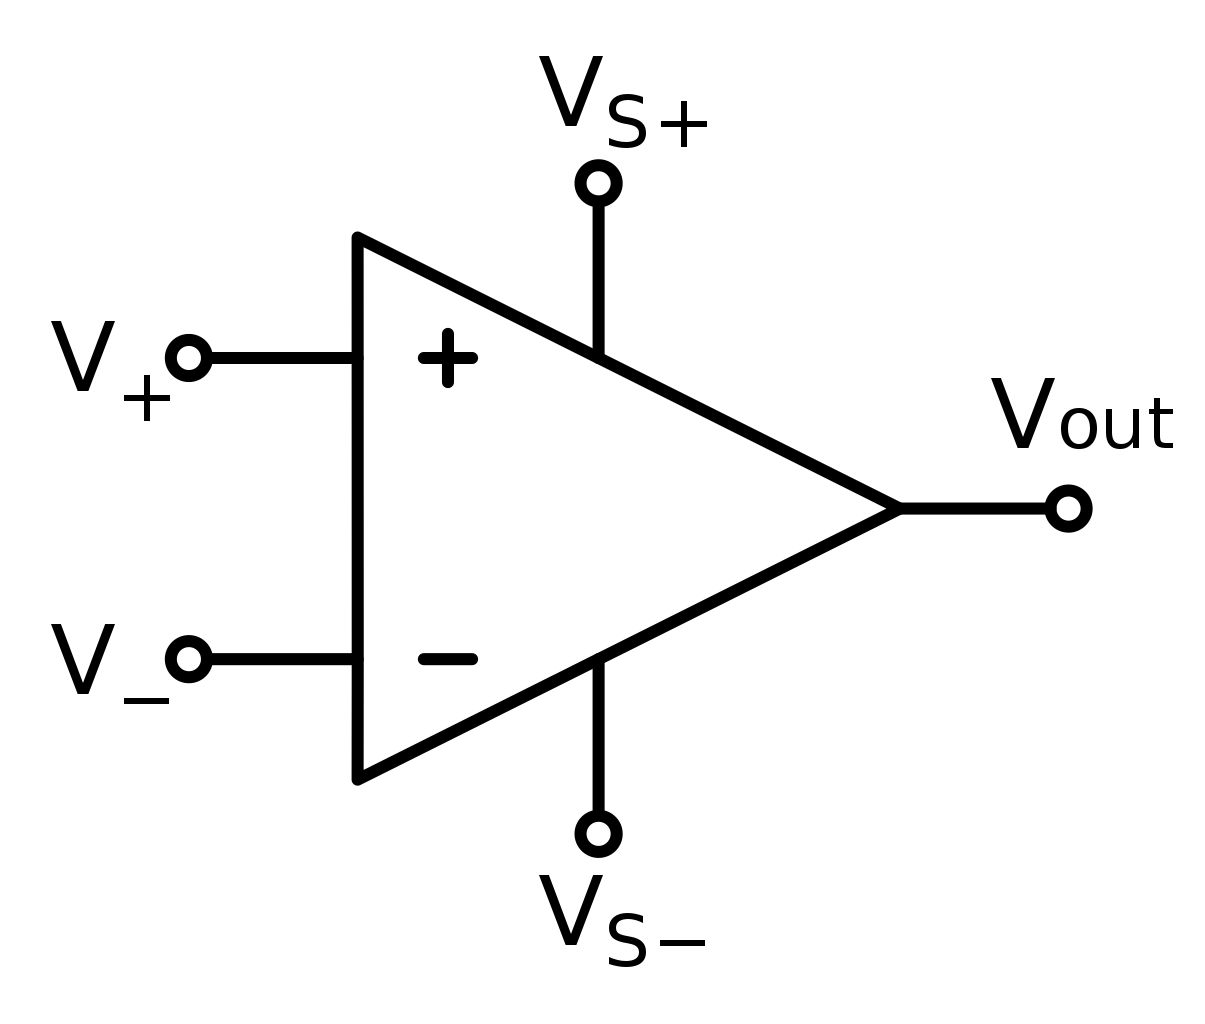
\includegraphics[width=40mm]{immagini/OpAmp1.png}
			\caption{Un OpAmp}
		\end{figure}
		L'OpAmp è in grado di amplificare il segnale per bene solo se $V_{S-}<A(V_+-V_-)<V_{S+}$, se per caso $A(V_+-V_-)>V_{S+}$, l'amplificatore porta $V_{out}$ al massimo voltaggio che può dare, cioè $V_{S+}$, e se $A(V_+-V_-)<V_{S-}$ $V_{out}=V_{S-}$.\newline

		Essendo $A$ molto grande basta una differenza di potenziale molto piccola ai capi dei terminali + e - per mandare l'OpAmp a $V_{S+}$ e $V_{S-}$, questo viene usato per dire in modo binario se un voltaggio è maggiore di un'altro voltaggio, infatti se $A|V_+-V_-|>>1$ si ha che $V_{out}=V_{S+}$ se $V_+>V_-$ e $V_{out}=V_{S-}$ se $V_+<V_-$.\newline

		Adesso che sappiamo ciò possiamo spiegare il secondo sottocircuito:
		Il secondo sotto circuito si può vedere nella figura \ref{fig:circ2}, il terminale positivo è collegato a $V_{sh}$ attraverso una resistenza di $100\Omega$, quindi visto che la corrente che passa per il terminale positivo è circa zero possiamo assumere che la differenza di potenziale ai capi sia trascurabile.\newline
		Chiamerò $V_P$\footnote{P sta per potenziometro} il potenziale che entra nel terminale negativo dell'OpAmp, esso è possibile regolarlo grazie al potenziometro che funge da partitore di tensione.\newline
		Essendo (quasi sempre) $A|V_{sh}-V_P|>>1$ si ha che 
		\begin{equation}
			\begin{cases}
				V_{discr}=V_C\textrm{ se } V_{sh}>V_P\\
				V_{discr}=V_E \textrm{ se } V_{sh}<V_E
			\end{cases}
		\end{equation}
		\begin{figure}
			\label{fig:circ2}
			\centering
			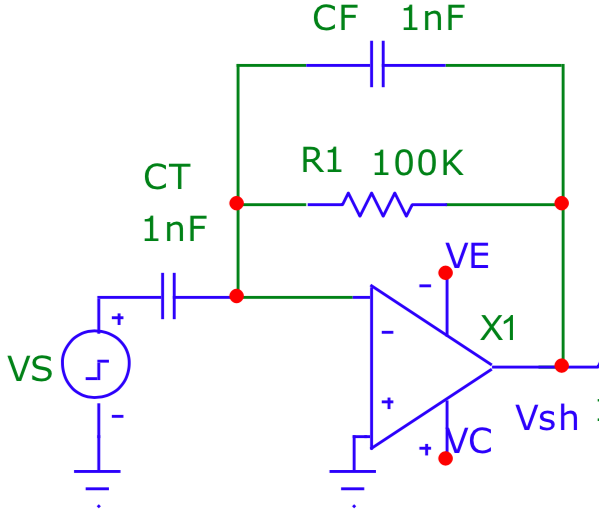
\includegraphics[width=70mm]{immagini/circ1b.png}
			\caption{secondo sotto-circuito}
		\end{figure}

		Unendo i due sottocircuiti come in figura \ref{fig:circ} si uniscono i risultati dei paragrafi precedenti:
		\begin{equation}
			V_{sh}=\vz e^{-t/C_FR_1}\quad \textrm{ e }\quad 
			\begin{cases}
				V_{discr}=V_C \textrm{ se } V_{sh}>V_P\\
				V_{discr}=V_E \textrm{ se } V_{sh}<V_E
			\end{cases}
		\end{equation}
		\begin{figure}
			\label{fig:circ}
			\centering
			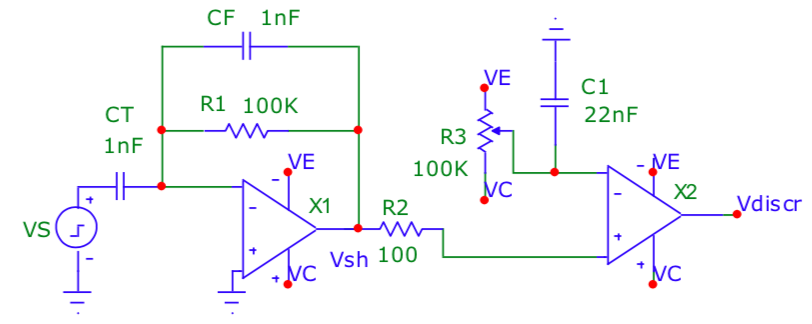
\includegraphics[width=120mm]{immagini/circa.png}
			\caption{Circuito}
		\end{figure}
		Se si vuole ricavare per quanto tempo $V_{discr}=V_C$ basta risolvere rispetto al tempo $V_{sh}>V_P$, quindi
		\begin{equation}
			\vz e^{-t/C_FR_1}>V_P\qquad-\frac{t}{C_FR_1}>\ln \bigg(\frac{V_P}{\vz }\bigg)\qquad t<C_FR_1\ln \bigg(\frac{2V_SC_T}{V_PC_F}\bigg)
		\end{equation}

	
	\subparagraph{c.}
		Per vedere la relazione tra durata del segnale in uscita e ampiezza del segnale in ingresso abbiamo tenuto $V_P=184.3\pm0.9 mV$ costante e abbiamo fatto variare l'ampiezza $V_S$, i dati raccolti sono mostrati in tabella \ref{tab:durata}. E' stato fatto anche un fit dei dati con la funzione $t=a \log(bx)$ lasciando $a$ e $b$ come parametri di fit (figura \ref{fit:1c}), per il fit non si sono considerati i punti in cui la durata del segnale in uscita è nulla, ovvero non è presente un segnale, in quanto questi punti vanno a formare una retta t=0 e non ha neanche senso parlare di durata del segnale di uscita.\newline
		Il fit  è stato fatto con absolute-sigma=False in quanto gli errori non sono statistici, i parametri risultano $a=(102.7\pm0.4)\mu s$ $b=8.02\pm0.09 V^{-1}$ con un $\chi^2_{ridotto}=0.036$, il chi quadro risulta basso probabilmente a causa della sovrastima degli errori di misura del voltaggio con l'oscilloscopio. Confrontando i parametri ottenuti con la teoria si ottiene che $a=(101.6\pm4.2)\mu s$ e $(b=10.1\pm0.5)V^{-1}$. $a$ è compatibile con i dati sperimentali, mentre $b$ non tanto...
	
		\begin{table}[h]
			\label{tab:durata}
			\begin{center}
				\begin{tabular}{cc}
					\hline
					$V_S [\mathrm{V}]$&$t[\mu s]$ \\
					\hline
					$(63.2\pm0.3) \mathrm{m}$ & $0$ \\
					$0.200\pm0.001$ & $0$ \\
					$0.412\pm0.002$ & $(1.23\pm0.01)\times 10^{2}$ \\
					$1.34\pm0.007$ & $(2.44\pm0.01)\times 10^{2}$ \\
					$3.32\pm0.02$ & $(3.36\pm0.02)\times 10^{2}$ \\
					$9.52\pm0.05$ & 	$(4.46\pm0.02)\times 10^{2}$ \\
					\hline
				\end{tabular}
			\end{center}
			\caption{Durata del segnale in uscita in funzione dell'ampiezza di $V_S$}
		\end{table}
		
		\begin{figure}
			\centering
			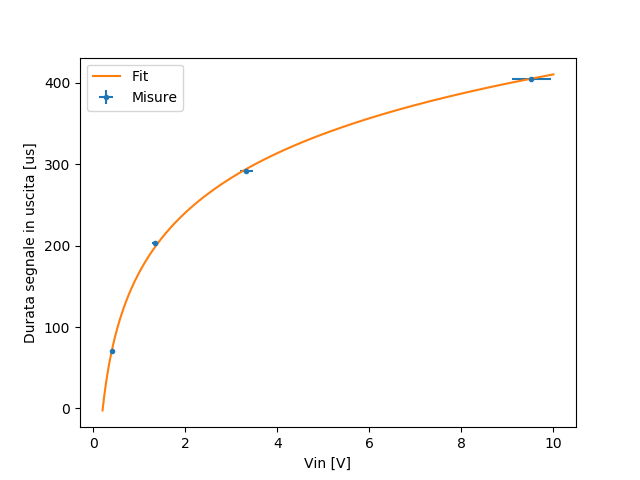
\includegraphics[width=\linewidth]{immagini/1c.png}
			\label{fit:1c}
			\caption{Fit della durata del segnale in uscita in funzione dell'ampiezza $V_S$}
		\end{figure}
		
		Facendo variare la tensione fornita dal potenziometro $V_P$ abbiamo misurato la minima tensione $V_S$ richiesta per avere un segnale $V_{discr}$, le misure sono riportate in \ref{tab 1c2}. Abbiamo anche eseguito un fit dei dati ottenuti con la funzione $f=a*x+b$ usando absolute-sigma=False, i parametri ottimali risultano $a=1.06\pm0.01$ $b=0.012\pm0.004 V$ con un $\chi^2_{ridotto}=0.09$, il chi quadro risulta basso probabilmente a causa della sovrastima degli errori di misura del voltaggio con l'oscilloscopio.
		\begin{table}
			\begin{center}
				\begin{tabular}{cc}
					\hline
					$V_P [\mathrm{V}]$&$V_{Smin} [\mathrm{V}]$ \\
					\hline
					$(184.3\pm0.9) \mathrm{m}$ & $(208\pm1)\mathrm{m}$ \\
					$0.308\pm0.002$ & $0.338\pm0.002$ \\
					$0.49\pm0.003$ & $0.54\pm0.003$ \\
					$0.937\pm0.005$ & $1.02\pm0.005$ \\
					$1.823\pm0.009$ & $1.92\pm0.01$ \\
					\hline
				\end{tabular}
			\end{center}
			\label{tab 1c2}
			\caption{Tensione minima per avere un segnale $V_{Smin}$ in funzione di $V_{P}$}	
		\end{table}
		
		\begin{figure}
			\centering
			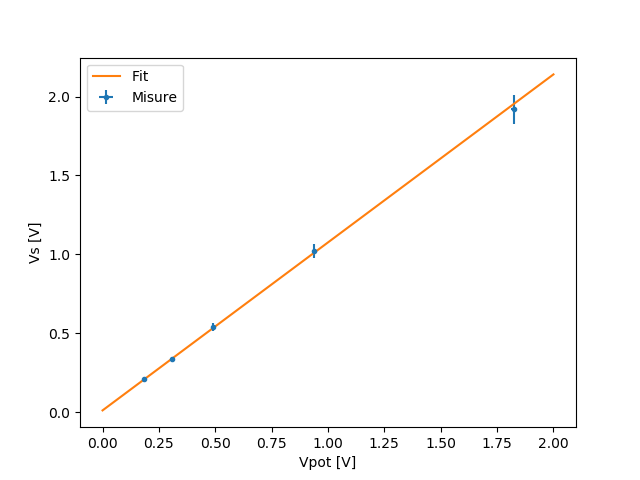
\includegraphics[width=\linewidth]{immagini/1c-2.png}
			\label{fit:1c-2}
			\caption{Fit della tensione minima per avere un segnale $V_{Smin}$ in funzione di $V_{P}$}
		\end{figure}
		\newpage



	\paragraph{2)}
	\subparagraph{a.}
		Partiamo dalle seguenti informazioni riguardanti il trigger di Schmitt (immagine \ref{fig:smith}): esso è uno squadratore d'onda, che funziona nel seguente modo:\newline
		\begin{figure}
			\label{fig:smith}
			\centering
			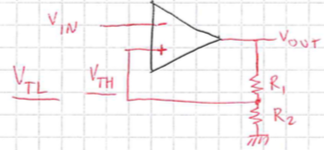
\includegraphics[width=70mm]{immagini/smitha.png}
			\caption{Trigger di Schmitt}
		\end{figure}
		\begin{equation}
			\begin{cases}
				V_{out}=V_{CE}\textrm{ se }V_->\frac{V_{CC}}{1+R_1/R_2}\\
				V_{out}=V_{CC}\textrm{ se }V_-<\frac{V_{CE}}{1+R_1/R_2}\\
				\textrm{se }\frac{V_{CE}}{1+R_1/R_2}<V_-<\frac{V_{CC}}{1+R_1/R_2}\textrm{ allora }V_{out}\textrm{ assume l'ultimo valore assunto}
			\end{cases}
		\end{equation}

		Il multivibratore astabile è mostrato in figura \ref{fig:multivibratore}, esso è un trigger di Schmitt con due diodi zener che limitano $-V_{br}<V_{out}<V_{br}$, dove $V_{br}$ è il voltaggio di breakdown degli zener. Inoltre grazie al passa-basso $V_-$ si carica dello stesso segno di $V_{out}$, ciò porta $V_-$ a raggiungere $V_+$.\newline
		Una volta che ciò succede, $V_+$ cambia di segno, e $V_-$ insegue $V_+$, tutto ciò crea un fenomeno oscillatorio.\newline
		\begin{figure}
			\label{fig:multivibratore}
			\centering
			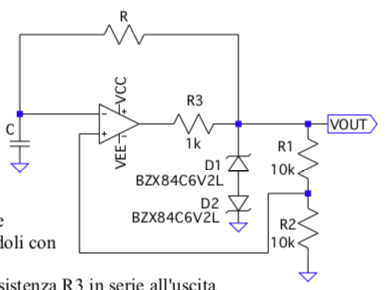
\includegraphics[width=100mm]{immagini/multivibratore.png}
			\caption{Multivibratore astabile}
		\end{figure}
		Il sistema che descrive il circuito è questo
		\begin{equation}
			\begin{cases}
				V_{out}-V_-=IR\\
				V_{out}-V_+=I_1R_1\\
				V_+=I_1R_2\\
				Q/C=V_-
			\end{cases}
			\begin{cases}
				V_{out}-V_-=IR\\
				\frac{V_{out}}{V_+}=\frac{R_1}{R_2}+1\equiv \alpha\\
				V_+=I_1R_2\\
				\frac{dV_-}{dt}=\frac{V_{out}-V_-}{RC}
			\end{cases}
		\end{equation}
		Supponiamo che a $t=0$ $V_{out}=V_{th}$ e $V_-=-\frac{V_{th}}{\alpha}$, risolvendo l'ultima equazione del secondo sistema si ottiene che\footnote{Viceversa se a $t=0$ $V_{out}=-V_{th}$ e $V_-=\frac{V_{th}}{\alpha}$ si ottiene $V_-=-V_{th}\bigg[1-\bigg(\frac{1}{\alpha}+1\bigg)e^{-t/RC}\bigg]$}
		\[
			V_-=V_{th}\bigg[1-\bigg(\frac{1}{\alpha}+1\bigg)e^{-t/RC}\bigg]
		\]		
		Per trovare il periodo dell'oscillazione basta imporre che 
		\[
			V_-=V_{th}\bigg[1-\bigg(\frac{1}{\alpha}+1\bigg)e^{-t/RC}\bigg]=\frac{V_{th}}{\alpha}
		\]
		risolvendo per t, e moltiplicanto per due equivale a trovare il periodo
		\[
			-(1+\alpha)e^{-t/RC}=1-\alpha\qquad -\frac{t}{RC}=\ln\frac{1-\alpha}{1+\alpha}\qquad t=\frac{\ln}{RC}\bigg(1+2\frac{R_2}{R_1} \bigg)
		\]
		\begin{equation}
			T=\frac{2}{RC}\ln\bigg(1+2\frac{R_2}{R_1} \bigg)
		\end{equation}
\end{document}








